\chapter{Dataset}

Why do we use a dataset?
- learning
- some research make them freely available to test

Describe how it was build ?

\textbf{UEC FOOD-100} and \textbf{UEC FOOD-256} are datasets used for food localization and recognition.

The UEC FOOD-100 dataset can be found in \footnote{Dataset can be found at \url{http://foodcam.mobi/dataset100.html}}. It was created in 2012 and presented in \cite{Matsuda2012a}.

It contains 100 types of food, mainly Japanese food. Each kind is represented by at least 100 samples.

\begin{figure}[h]
    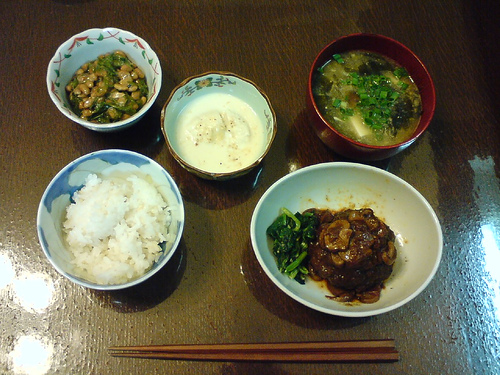
\includegraphics[width=8cm, height=8cm]{img/multiple_food_items_1}
    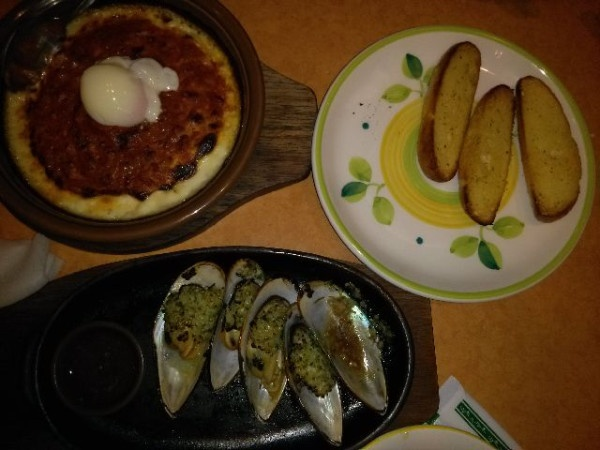
\includegraphics[width=8cm, height=8cm]{img/multiple_food_items_2}
    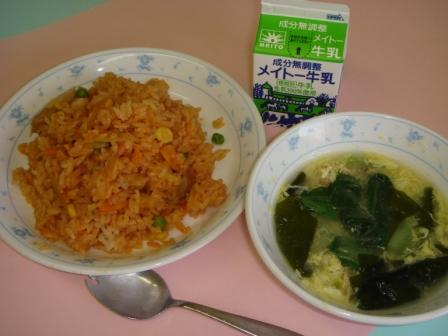
\includegraphics[width=8cm, height=8cm]{img/multiple_food_items_3}
    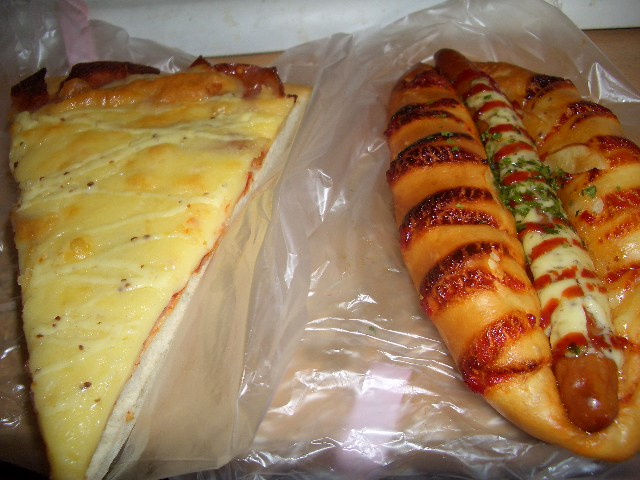
\includegraphics[width=8cm, height=8cm]{img/multiple_food_items_4}
    \caption{Example of pictures with multiple food items from UEC FOOD 256}
    \label{fig:presentation_multiple_food_items}
\end{figure}

As presented in figure \ref{fig:presentation_multiple_food_items}, a photo can contain more than one food items. The dataset contains files to indicate bounding boxes marking the location of a food items.

UEC FOOD-256 can be found in \footnote{Dataset can be found at \url{http://foodcam.mobi/dataset256.html}}. It was presented in \cite{Kawano2015} in 2015. It contains  the 100 types of food from UEC FOOD-100 plus 156 new ones. The newly introduced food kinds are more international dishes with food from various countries such as France, Italy, the USA, China, Thailand, Vietnam, Japan and Indonesia. As for FOOD 100, every food photo has a bounding box indicating the location of the food item.

The most represented category is miso soup with 728 and rice with 620 pictures.